\documentclass[a4paper, 11pt]{article}
\usepackage{comment} % enables the use of multi-line comments (\ifx \fi) 
\usepackage{lipsum} %This package just generates Lorem Ipsum filler text. 
\usepackage{fullpage} % changes the margin
\usepackage{graphicx}

\begin{document}
%Header-Make sure you update this information!!!!
\noindent
\large\textbf{Specification of a bachelor thesis} \hfill \textbf{Adam Kasperowicz} \\

\section*{Topic}
The aim of the thesis will be a construction of a decentralized loan system using Ethereum technology. The final product should be a proof of concept of the possibilities of blockchain and smart contracts technologies. 

\section*{Problem}
Loan business is a vital part of the modern financial world. Being one of the oldest financial mechanisms to exist it provides the consumers with required capital. Throughout the whole history it has always been an example of a centralized system. That is one central entity hoarding the money from different sources gets inquired about financing possibilities. Such entity is in power to decide upon who shall receive the funding and with what interest. It is also the burden of the entity to deal with any cases of loan repayment disobedience.

The are a few problems with this concept all of which stem from the design itself. Firstly, if one wants to capitalize on his spare money through this type of scheme he has to create an entire new company with all the legal requirements and an administrative burden. Secondly, all the processes such as storage of money, allocation of loans, interest serving, acceptance of clients etc. have to be taken care of by the workers of the loan company. Thus, costs are generated and sources of human errors and introduced. Lastly, due to the way financial services are diversified around the world it is often very troublesome or even impossible to service loans internationally.

\section*{Solution}
All of the aforementioned disadvantages can be circumnavigated using the fruits of modern computer science. That is blockchain and tightly related smart contracts. A Decentralized Autonomous Organization(DAO) is introduced which serves as a medium between those who have the capital and those who need the capital. The DAO which acts as a loan system allows anyone with any amount of Ethereum to bid a loan with an arbitrary duration and interest on a public exchange. At the same time a counterparty publishes an ask offer stating how big of a loan is required under specific duration and interest. The whole process closely resembles stock exchange. In result market forces lead to an equilibrium allowing both parties to reach their goal. The exchange itself is based on blockchain and no central server is required.

This design solves all of the issues pointed out so far. Anyone in the whole world with a connection to an internet is able to put his money to good use with few mouse clicks while maintaining anonymity. All of the operational activities are also immediately eradicated by market forces backed by smart contracts. Of course the problem of loan repayment still remains but the possible solutions of this specific mischief will be explained in the section describing a loan taker.

\section*{Loans}
One loan offer on an exchange will consist of following parameters:
\begin{itemize}
\item \textbf{Basis}: Size of the loan denominated in Ethereum.
\item \textbf{Duration}: The time after which the whole loan should be paid back together with interest.
\item \textbf{Interest}: Percentage of the loan basis which has to be additionally paid by loan taker.
\item \textbf{Collateral}: Information whether the loan is backed by a third party and has a low probability of going default. For example loan taker with no evidence to back his repayment probability will have only access to loans with collateral parameter being equal to None. At the same time loan taker with his loan being backed by a special bank agreement whereas there is a deposit with amount equal to the loan basis and interest incurred which is connected to a smart contract will have access to loans with collateral being equal to Yes.
\end{itemize}

The process of buying and selling loans will have the same characteristics as the one seen on the stock exchange. 

That is loan ask whose size exceeds size of one respective loan bid will automatically cover the second identical loan bid. For example loan taker A asks for a loan of 1 ETH. There are two identical offers by loan provider B and C both equal to 0.5 ETH. The matching will automatically buy for A both loans from B and C.

Moreover, if loan taker asks for a loan of interest higher than the lowest present on the market he will be sold the loan with the lowest interest. For example loan taker asks for a loan of interest 2\%. There are loans on the market being bid with both interest of 2\% and 1\%. The loan of 1\% will be sold to the loan taker.


\section*{Types of users}
The project provides for three types of possible actors. They are as follows:
\begin{itemize}
\item \textbf{Loan providers}: Any user with spare Ethereum and access to the application. Such person bids his loan offer and once the loan is sold automatic processes backed by smart contracts care for repayments.
\item \textbf{Loan takers}: User who has fulfilled required information inquires and can be assured of that at least one of the methods of repayment can be exercised on him. The methods are:
\begin{enumerate}
\item Regular individual refilling of his repayment account.
\item Usage of a collateral deposit from a third party.
\item Following legal procedures by bailiff of a country where the loan taker is located.
\end{enumerate}
\item \textbf{Authorities}: Third parties which for example serve the role of a collateral deposit or bailiff chasing the loan taker. This user has the possibility to refill the account of the loan takers repayment account.
\end{itemize}

\section*{Processes}
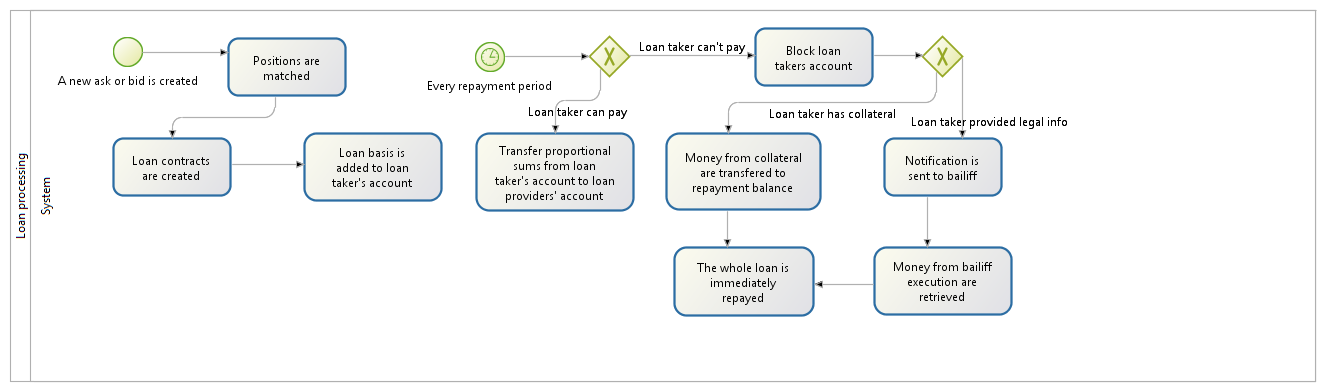
\includegraphics[width=\textwidth]{images/Loan_processing-1_0.png}
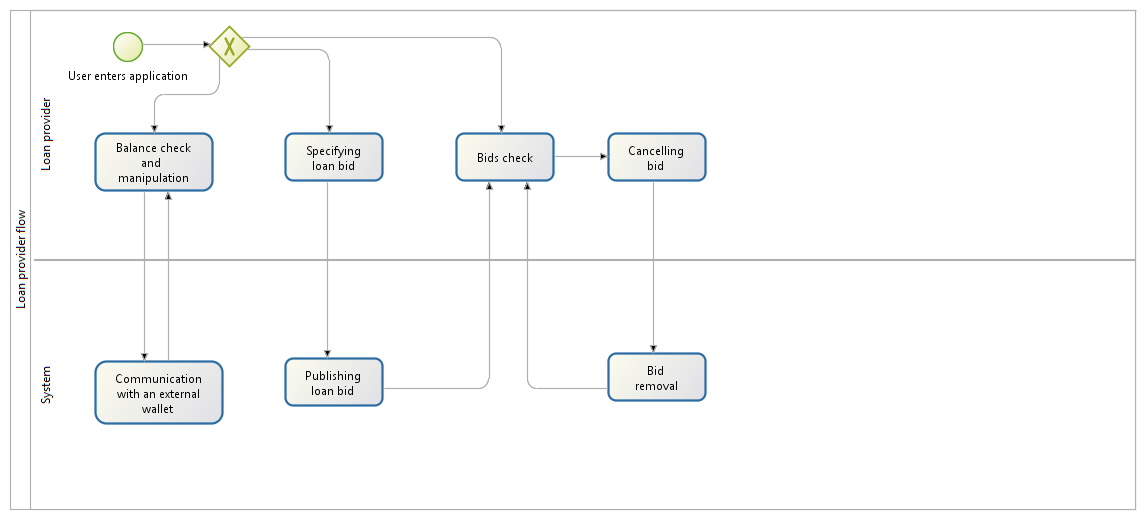
\includegraphics[width=\textwidth]{images/Loan_provider-1_0.png}
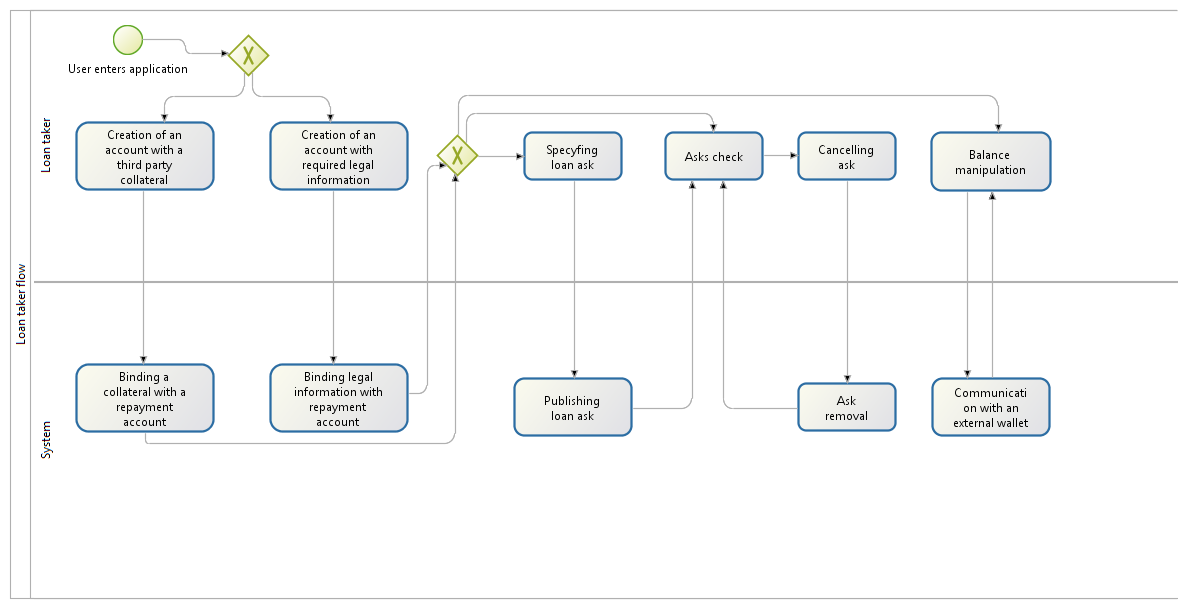
\includegraphics[width=\textwidth]{images/Loan_taker-1_0.png}
\newpage

\section*{Requirements}
The complete system should provide following functions:
\begin{enumerate}
\item Loan providers and loan takers should be able to:
\begin{itemize}
\item check and transfer funds to and from their accounts using external wallet based on Ethereum network.
\item specify the following parameters in their loan bids and asks: Basis, Duration, Interest, whether it has collateral.
\item check their open bids and asks as well as the whole public exchange.
\item cancel all of their open bids and asks.
\end{itemize}
\item Loan takers should be able to:
\begin{itemize}
\item specify legal informations which could be used by bailiff if repayment did not happen. At the same time the information should remain confidential so long there is no need to use them.
\item bind his account with an account of a third party. The additional account will always hold a sum required to repay the whole loan when needed.
\end{itemize}
\item Every user should be able to:
\begin{itemize}
\item access the application having only internet connection.
\item maintain his anonymity while using the system.
\end{itemize}
\end{enumerate}
\section*{Architecture}
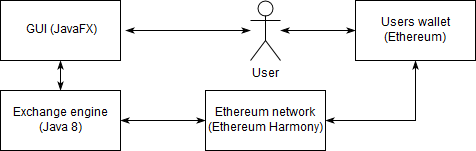
\includegraphics[width=\textwidth]{images/Loan.png}
The diagram presents parts of the application and the respective technologies used to implement them.The whole projects is based on Java and its libraries binding it with Ethereum network.  

\section*{Visual design}
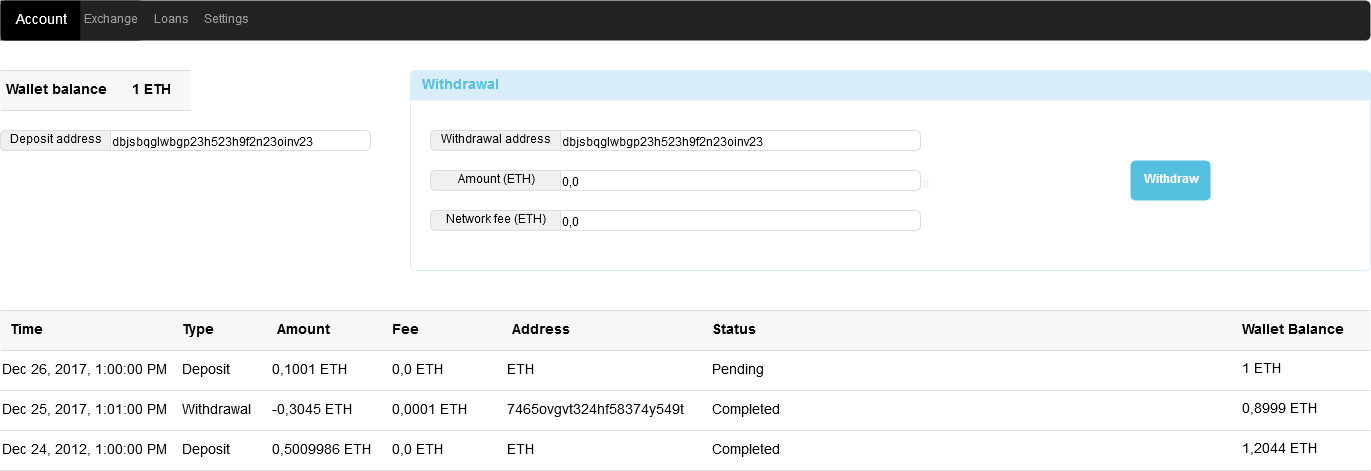
\includegraphics[width=\textwidth]{images/Account_window.png}
\hfill
\\
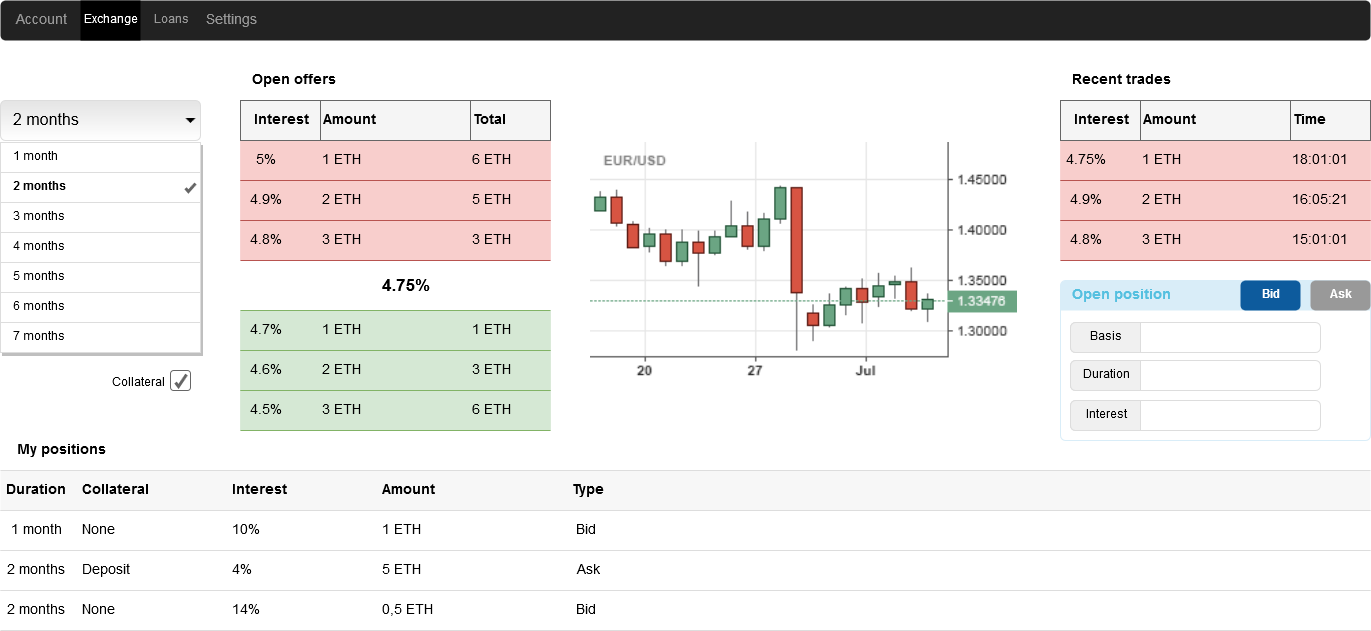
\includegraphics[width=\textwidth]{images/Main_window.png}
\hfill
\\
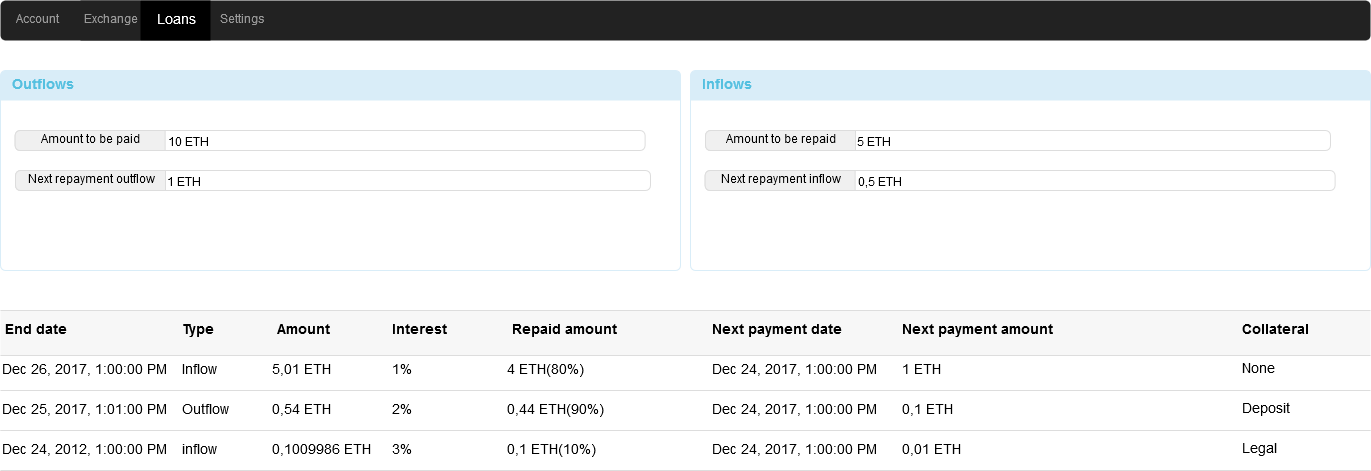
\includegraphics[width=\textwidth]{images/Loans_window.png}
\hfill
\\
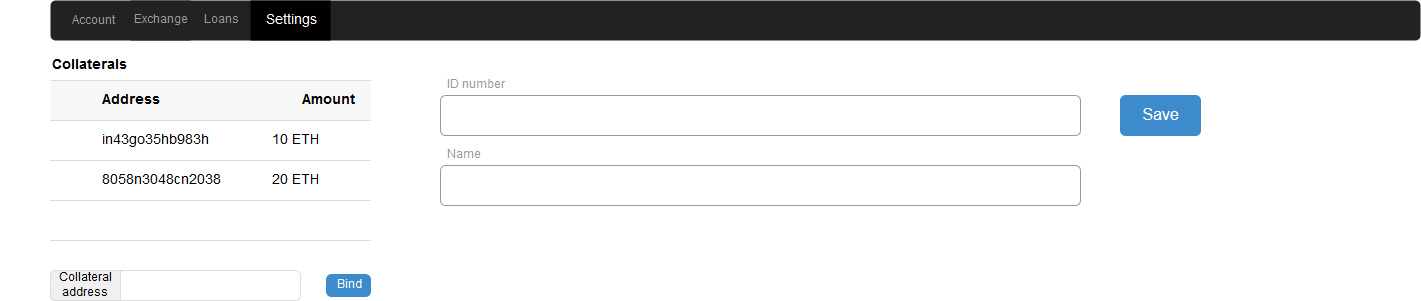
\includegraphics[width=\textwidth]{images/Settings_window.png}

\section*{Implementation steps}
\begin{enumerate}
\item Deployment of a test Ethereum network.
\item Construction of smart contracts backing loans.
\item Construction of a matching engine for exchange.
\item Creation of users.
\item Integration of collateral possibilities.
\item Construction of a graphical user interface.
\end{enumerate}

\end{document}
